\section{Clustering Analysis}
\label{sec:clustering}

Given extracted feature data, we can model features' distributions, fit DP mixtures, fit Markov chain and eventually make implications on the results (process 2-5.1 in the modelling pipeline in \Cref{tab:pipeline}). Before that, we would like to make assumption on customer month independence and verify it through data.

\subsection{Customer Month Independence}

How does cancellation rate change over time? To see this, we group subscribers by customer month and calculate the number of each group. Suppose there are $n_t$ pupils in customer month $t$ for $t=1,\dots,T$, then the cancellation rate at $t$ is defined as $1-n_{t-1} / n_t$ for $t=2,\dots, T$. Recall from section \ref{sec:dataScope} that $n_1 = 2672$ and $T = 49$. We plot the evolution of number of subscribers and cancellation rate in \Cref{fig:cancellationRate}.

\begin{figure}[!h]
\centering
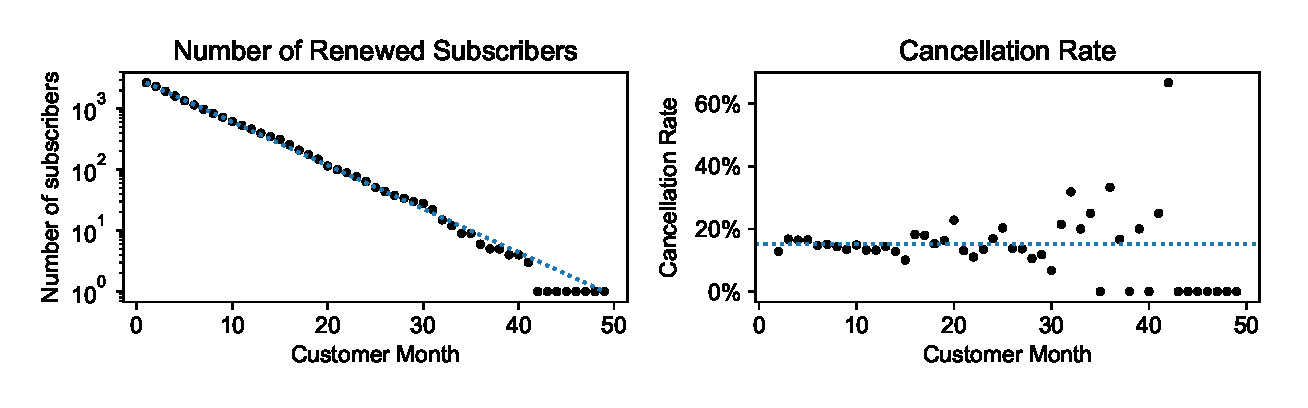
\includegraphics[scale=.7]{CancellationRate.eps}
\caption{Evolution of subscriber number and cancellation rate.}
\label{fig:cancellationRate}
\end{figure}

The vertical axis of the subscriber number plot is log-scaled. We observe that the subscriber numbers over time fit a straight dashed line very well, inferring the number is exponentially decreasing. This is again verified by a relatively constant cancellation rate over time. There comes a lot of noises when customer month is larger than 25, because after that the number of live subscribers has reduced to less than 50 so noise dominates the estimate.

Within each customer month we can assume each customer in independent from others, then we can interpret the churn rate of the customer month group as the churn probability of each individual in that group. Hence, this observation leads to a very important assumption which greatly simplifies our model: each customer's cancellation outcome is only dependent on his features within the current customer month, not further previous ones. In other words, customer months are independent in leading to churn outcome, so we can consider all customer months together and perform a single clustering. %This again implies that the Markov chain is stationary, which means $A_1 = \cdots = A_T$.

As a result, in the following analysis, we will stack feature data time series $\left\lbrace \mathbf{X}_1, ~\mathbf{X}_2, ~\dots, ~\mathbf{X}_t, ~\dots, ~\mathbf{X}_T \right\rbrace$ into a single matrix $\mathbf{X} \in \mathbb{R}^{m \times n}$ with $n = \sum_{t=1}^{T} n_t$. We compute that $n=17861$.

\subsection{Distributional Modelling of Features}

We move to find appropriate density form $\phi(\cdot)$ for all $m=15$ features. We will have a visual check of their empirical distributions and also consider their correlation structure. However, we have to firstly tackle with missing data problem introduced by the way we construct features.

\subsubsection{Features with Missing Data}

It is not uncommon to observe pupils who have no visits to the service at all within a customer month although they are still in subscription. This introduces missing information to features such as mark, fail rate, etc.. We cannot simply fill these information by zeros, which are indistinguishable from real zero marks obtained by other pupils and will servrely distort the distribution if their number is large. 

We solve this problem by splitting pupils into three group partitions according to their activity level, where clustering task will be performed on different groups with different sets of features. The selection of features in each group ensure that there is no missing information or trivial information (for example, we can ignore ``number of visit'' as a feature for pupils who have no visits). We list the group definition and the associated churn rate and size in \Cref{tab:G123}. This simple splitting can already form clusters of very different churn rates. 

\begin{table}[!h]
\centering
\footnotesize
\begin{tabular}{c|p{9cm}|c}
\hline
\textbf{Group} & \textbf{Description} & \textbf{Churn rate (Size)}\\
\hline
G1 &
\textbf{Inactive:} pupils having no visits at all within the customer month. &
22.99\% (6417) \\
\hline
G2 &
\textbf{No-assess:} pupils having visits, but only take replay mode and do not take any exercise/lesson (which will give marks, pass/fail outcome) at all within the customer month. &
16.94\% (425) \\
\hline
G3 &
\textbf{Complete Info:} pupils having visits, and have taken exercise/lesson within the customer month. &
10.21\% (11019) \\
\hline
\end{tabular}
\caption{Group partitions of pupils due to activity level.}
\label{tab:G123}
\end{table}

\subsubsection{Independent and Multivariate Features}

The simplest form for $\phi(\cdot)$ is multivariate Gaussian where each individual feature is assumed to be a mixture of normal distributions. This appears unrealistic, even after the Box-Cox transformation. We display the empirical distributions for all features in \Cref{fig:featureDistribution}. The four ``rate'' features at the top apparently violate the Gaussian mixture assumption. The problem comes from the phenomenon called single-value-inflation, where a single value such as 0 has significantly frequent observations. In fact, mixture model is an ideal for modelling such distribution since it allows the overall distribution to be consisted of several different simpler distribution (not only Gaussian). We can model this feature separately from other features by assuming that it is independent of other features.

\begin{figure}[!h]
\centering
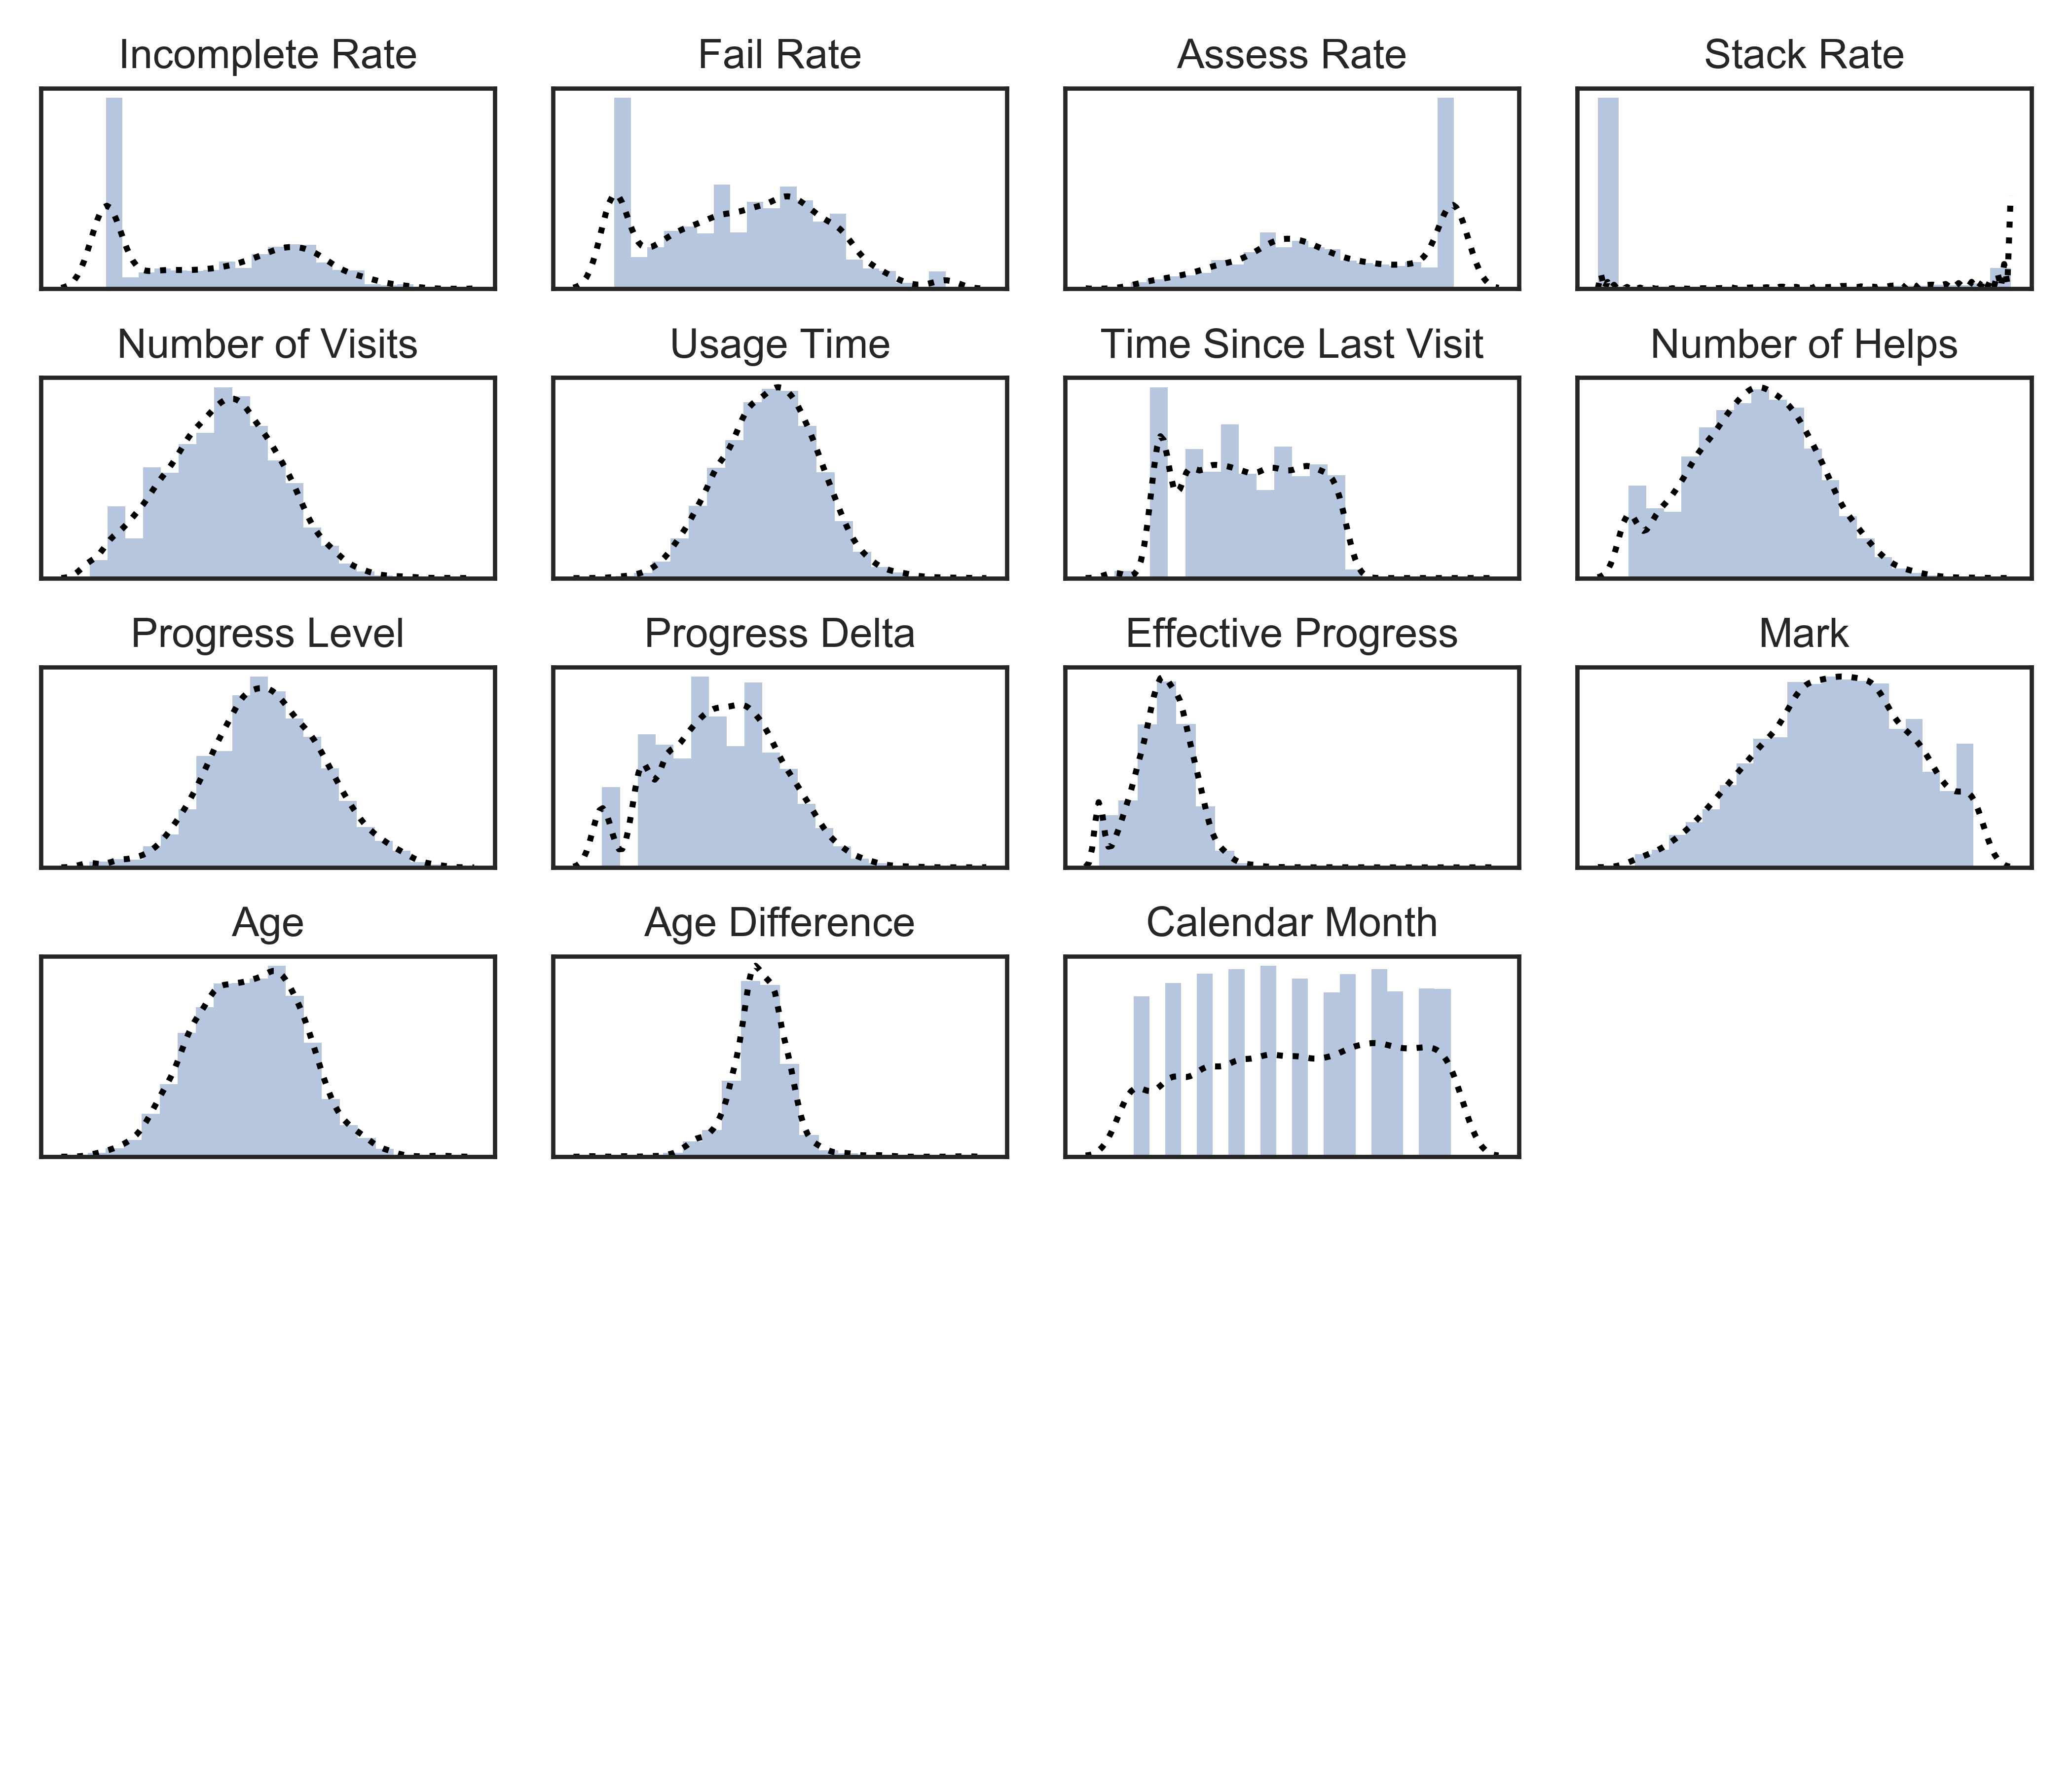
\includegraphics[scale=.7, trim={0 6cm 0 0}, clip]{FeatureDistribution.eps}
\caption{Empirical distribution (histogram) and Gaussian kernel for all features in G3.}
\label{fig:featureDistribution}
\end{figure}

Hence, we want to assume the four ``rate'' features to be independent from other features, and thereafter fit bespoke mixtures for each. But how likely the independence assumption holds true? We can assess the independence by at least look at the correlation structure of all features, as shown in \Cref{fig:featureCorrelation}. Incomplete rate and assess rate are very negatively correlated, but uncorrelated with other features. Fail rate and stack rate have slightly negative correlation with mark, and uncorrelated with others. Overall it seems valid to model these 4 features separately from other features, and all the other 11 features will be modelled using the multivariate Gaussian mixtures (where the dependence structure will be preserved).

\begin{figure}[!h]
\centering
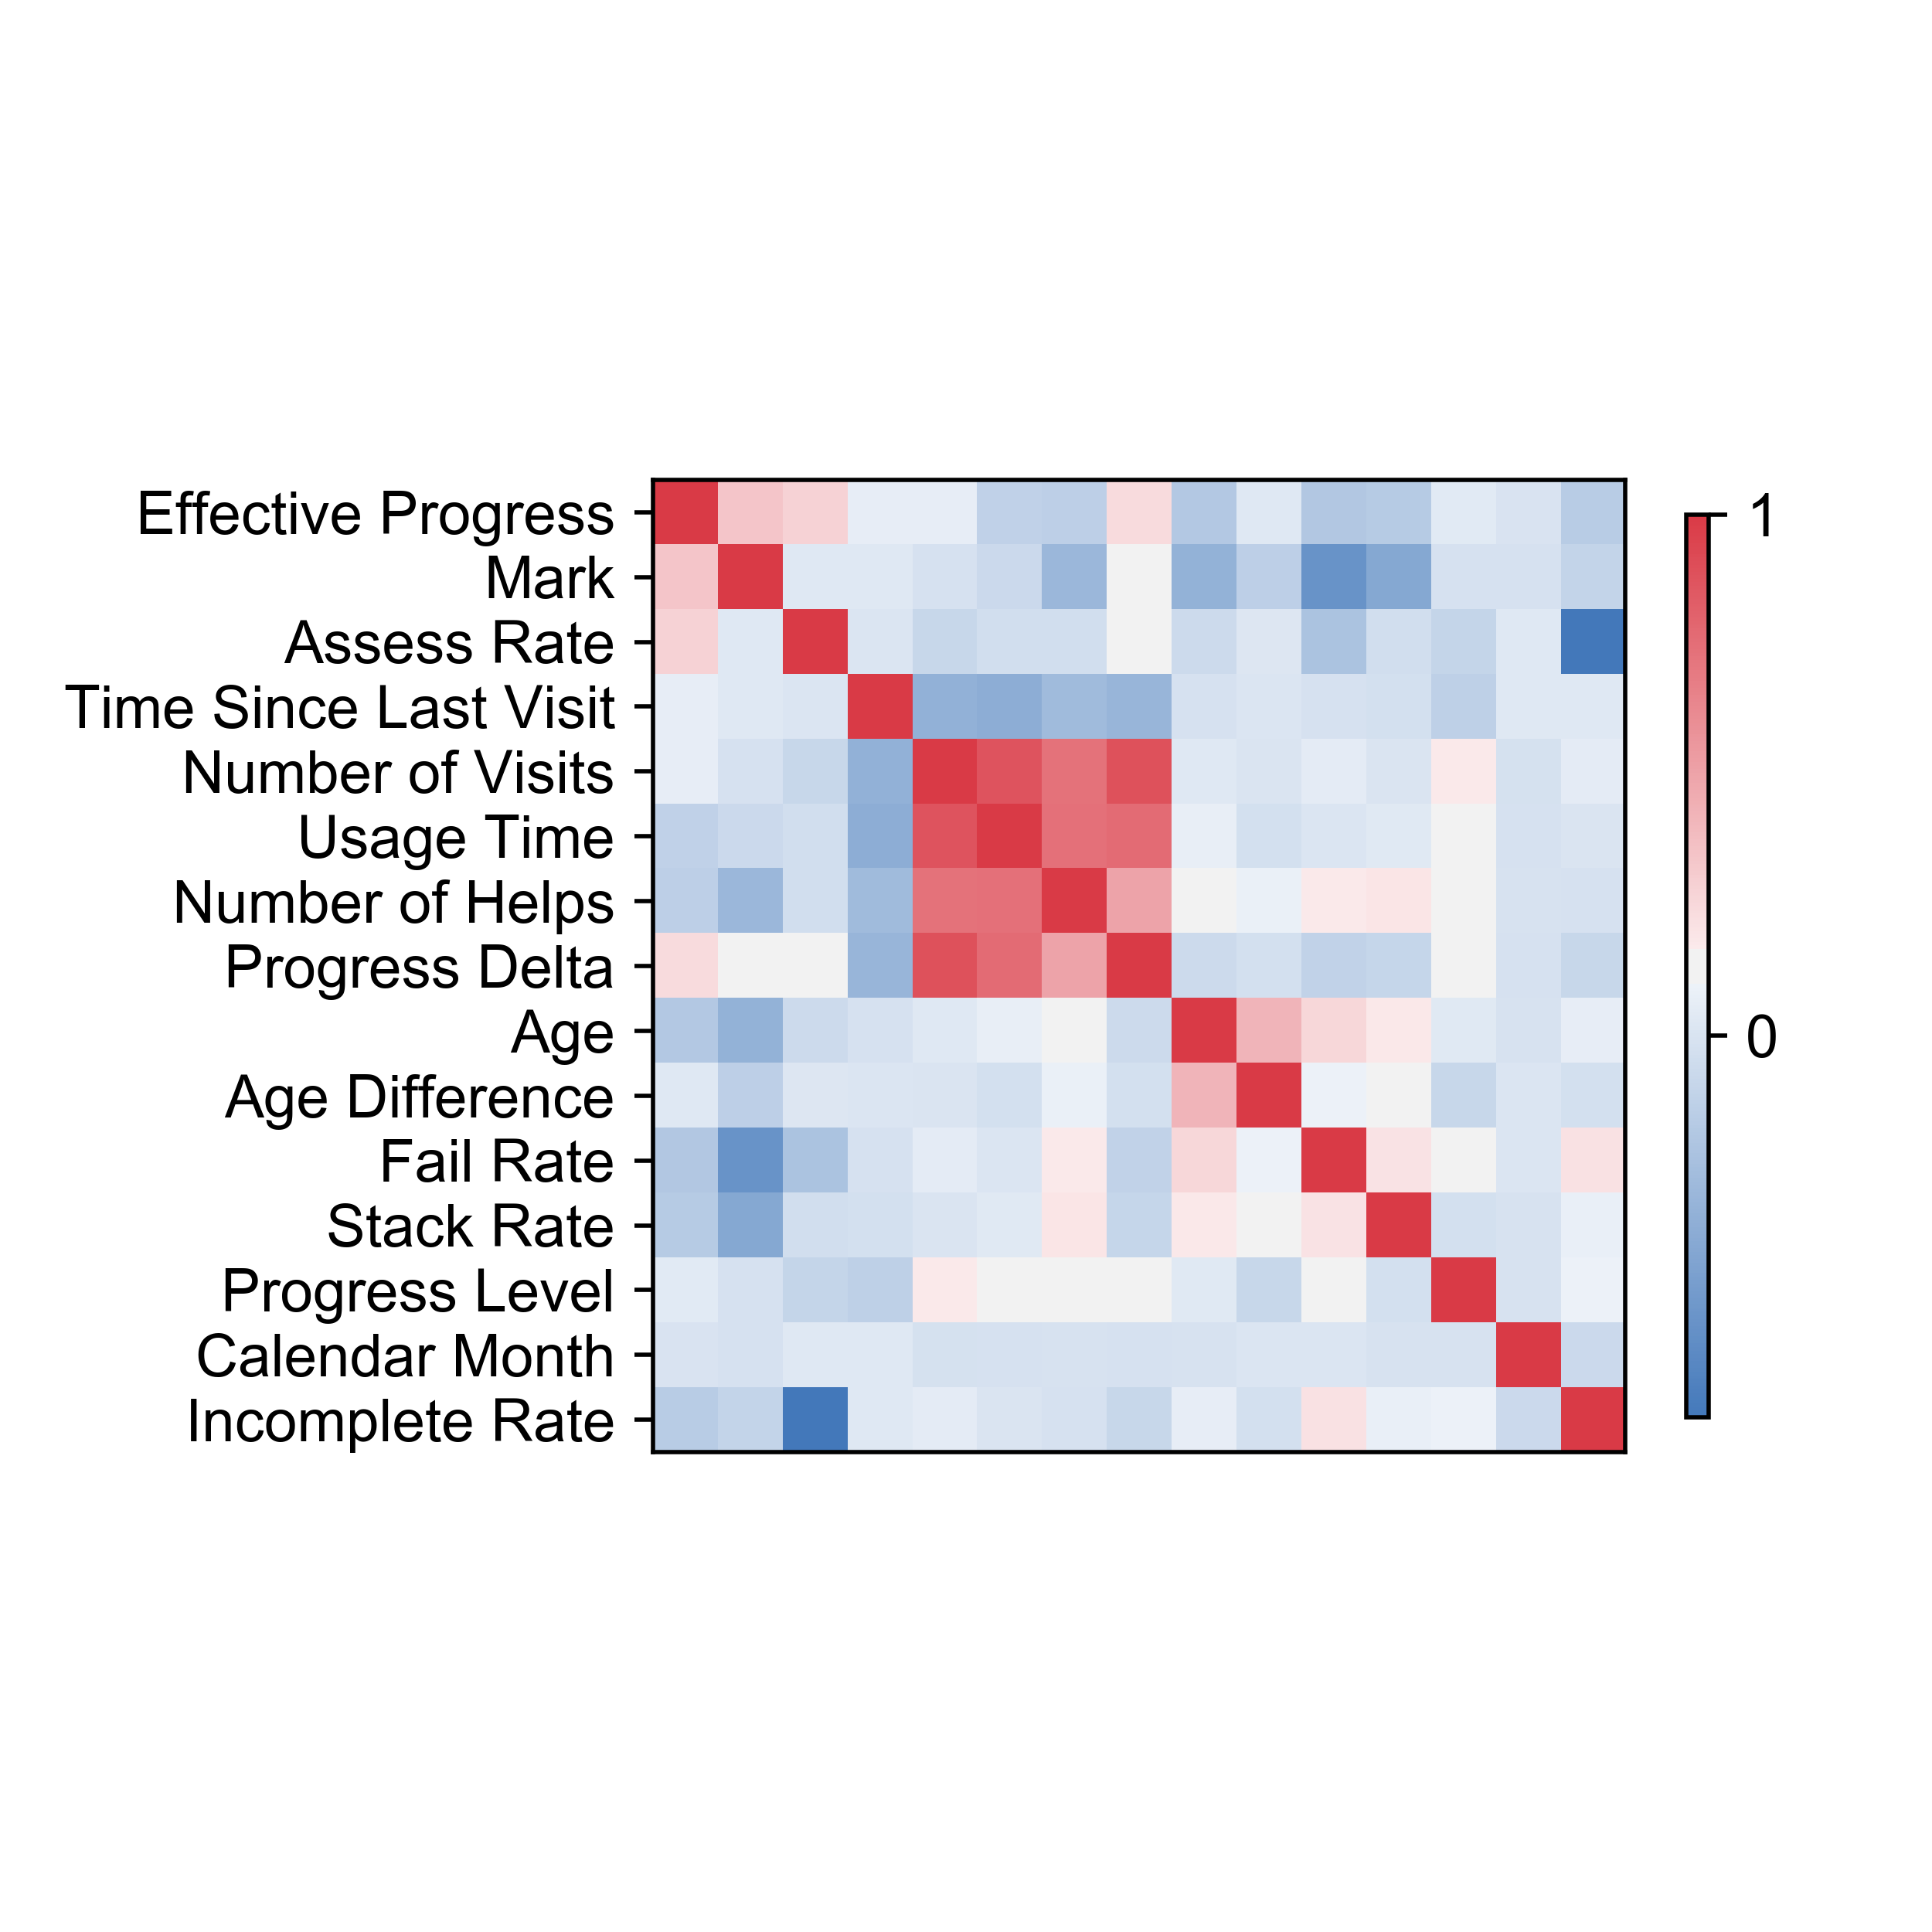
\includegraphics[scale=.7, trim={0 2.5cm 0 2.5cm}, clip]{FeatureCorrelation.eps}
\caption{Correlation of all features. Red stands for perfect positive correlation, blue for perfect negative correlation and white for uncorrelation.}
\label{fig:featureCorrelation}
\end{figure}

To choose the suitable mixture form for each independent feature, we have a visual check on its empirical distribution and decides the type of simple distribution and the number of components. The fitting result from EM-algorithm is visualised in \Cref{fig:fitIndependentFeature}.

\begin{figure}[!h]
\centering
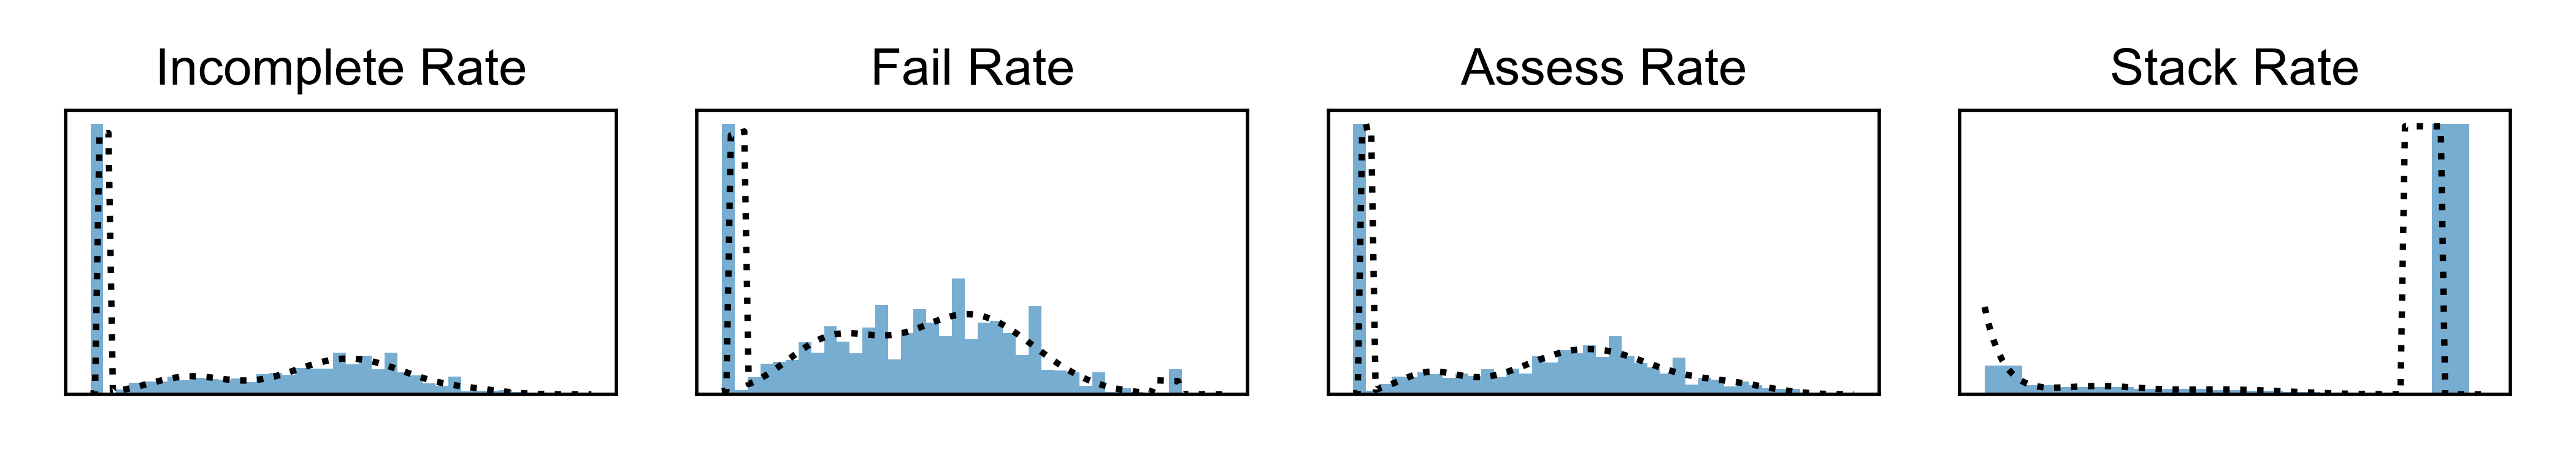
\includegraphics[scale=.7, trim={0 0 0 0}, clip]{FittingIndependentFeatures.eps}
\caption{Fitting bespoke mixture model for independent features. Assess rate and stack rate data are reversed by their order to have a better fitting to simple distribution. This is achieved by linear transformation as described in (\ref{eq:linearTransformation}). We can see how this outperforms compared with the Gaussian kernel for these features in \Cref{fig:featureDistribution}. }
\label{fig:fitIndependentFeature}
\end{figure}

The choice of component distributions and their quantities are listed in \Cref{tab:fitIndependentFeature}. Note that for independent features we do not infer the number of clusters from data following Baysian approach. The reason is exactly why we assume their independence from other features and model them separately: they have idiosyncratic distributions so we want to have special treatment to capture them. The side effect is the component choice might be sensitive to observed data, and anytime when new data come in we need to verify that the choice is not severely violated. Otherwise we need alter to a more suitable component choice. Fortunately, the component choice listed in \Cref{tab:fitIndependentFeature} works well for both G2 and G3 data (G1 has none of the ``rate'' features defined by construction). For each component, EM-algorithm will estimate (1) the parameters of each component distribution ($\lambda$ for exponential, $(\mu, \sigma)$ for Gaussian, etc.) and (2) the weights of each component by (locally) maximising the likelihood.

\begin{table}[!h]
\centering
\footnotesize
\begin{tabular}{p{3cm}|p{7cm}}
\hline
\textbf{Feature} & \textbf{Component distribution (Number)} \\
\hline
Incomplete rate &
Uniform (1), Gaussian (3) \\
\hline
Fail rate &
Uniform (2), Gaussian (2) \\
\hline
Assess rate &
Uniform (1), Gaussian (3) \\
\hline
Stack rate &
Exponential (1), Uniform (1), Gaussian (2) \\
\hline
\end{tabular}
\caption{Component distributions and their quantity in mixture models for each independent feature.}
\label{tab:fitIndependentFeature}
\end{table}

In summary, we split the set of $m=15$ features, by idiosyncratic attributes exhibited in their empirical distribution, into a set of $m_\mathcal{I} = 4$ independent features and $m_\mathcal{M} = 11$ multivariate Gaussian features. Let's denote the density forms for independent features as $\phi_{\mathcal{I}_i} (\cdot) : \mathbb{R} \mapsto \mathbb{R}$ for $i = 1,\dots, m_\mathcal{I}$, and the one for multivariate features as $\phi_\mathcal{M} (\cdot) : \mathbb{R}^{m_\mathcal{M}} \mapsto \mathbb{R}$. Hence, the aggregated density form is
\begin{equation}
\phi(\cdot) = \prod_{i=1}^{m_\mathcal{I}} \phi_{\mathcal{I}_i} (\cdot) \phi_{\mathcal{M}}(\cdot),
\end{equation}
where the multivariate density is a mixture of multivariate Gaussian parametrised by weights $\bm\pi$ and mean-variance pair $(\bm\mu, \bm\Sigma)$.

\subsection{Fitting Dirichelet Process Mixtures}

We then fit the $m_\mathcal{M}$ multivariate features by Dirichelet process mixtures, which will give estimates of weights $\bm\pi$ and posterior distribution of the Gaussian mean-variance pair $(\bm\mu, \bm\Sigma)$.

A prior distribution for $(\bm\mu, \bm\Sigma)$, which is previously denoted as $G_0$ the base measure in DP, has to be pre-defined. In addition, the DP weight concentration parameter $\alpha$, and the maximum number of clusters $K_\text{max}$ need be specified. These are a part of model parameter choice. We list our choice in \Cref{tab:DPFittingPrior}.

\begin{table}[!h]
\centering
\footnotesize
\begin{tabular}{l|l}
\hline
\textbf{Parameter} & \textbf{Value} \\
\hline
$\alpha$ &
$1/m_\mathcal{M}$ \\
Prior of $\bm\mu$ &
Gaussian(mean = sample mean, covariance = identity matrix) \\
Prior of $\bm\Gamma$ &
Wishart(degree of freedom = $m_\mathcal{M}$, covariance = sample covariance) \\
$K_\text{max}$ &
30 \\
\hline
\end{tabular}
\caption{Parameter choice for DP mixture model.}
\label{tab:DPFittingPrior}
\end{table}

We use the variational inference presented by Blei and Jordan \cite{blei2006}. An example result is shown in \Cref{fig:clusteringG3}. Though $K_\text{max}=30$ are pre-defined as a upper boundary for number of components, the feature data only infer 4 clusters. We count the size of each cluster and compute the churn rate for each cluster by formula (\ref{eq:clusterChurn}).

\begin{figure}[!h]
\centering
\includegraphics[scale=.7, trim={0 0 0 0}, clip]{ClusteringG3.eps}
\caption{Identified clusters by multivariate features in G3, their sizes and associated churn rate. The clustering result is a local optimism which is dependent on the initialisation fed into the numerical procedure. Here we show one instance. The two plots show exactly the same thing but with different scales of vertical axis. Cluster sizes can be easily compared in left plot while it is easier to compare cluster churn rate in right plot. The dashed line in right plot indicates the group-level churn rate for G3.}
\label{fig:clusteringG3}
\end{figure}

Both cluster size and churn rate show sensible patterns and have meaningful implications:
\begin{itemize}
\item The purely behaviour-based model can infer clusters with very different churn rate. The highest cluster churn rate is 2.6 times higher than the lowest one, and 2.2 times higher than the group average.
\item It is more challenging to identify pupils of higher churn probability, reflecting by the observation that the higher rate, the smaller cluster is found.
\end{itemize} 

We need combine the clusters from independent and multivariate features together. By our component distributions configuration in \Cref{tab:fitIndependentFeature}, modelling each independent feature can find 4 clusters. Plus the 4 clusters identified from the multivariate features, our model can identify up to $1024 = 4^5$ possible clusters. Nevertheless, it ends up with 268 clusters found in G3. The average size and cluster churn rate are shown in \Cref{fig:clusteringG3Complete}. By ``average'', we compute the average size of clusters with the same churn rate. The model identifies a couple of clusters with 100\% and 0\% churn rate. However, the cluster size is really small for those extreme high/low churn rate. This implies that it is much easier to identify ``normal'' customers where the churn probability is around population average, but really challenging to distinguish ``risky'' or ``safe'' customers who have very high or low chance to cancel.

\begin{figure}[!h]
\centering
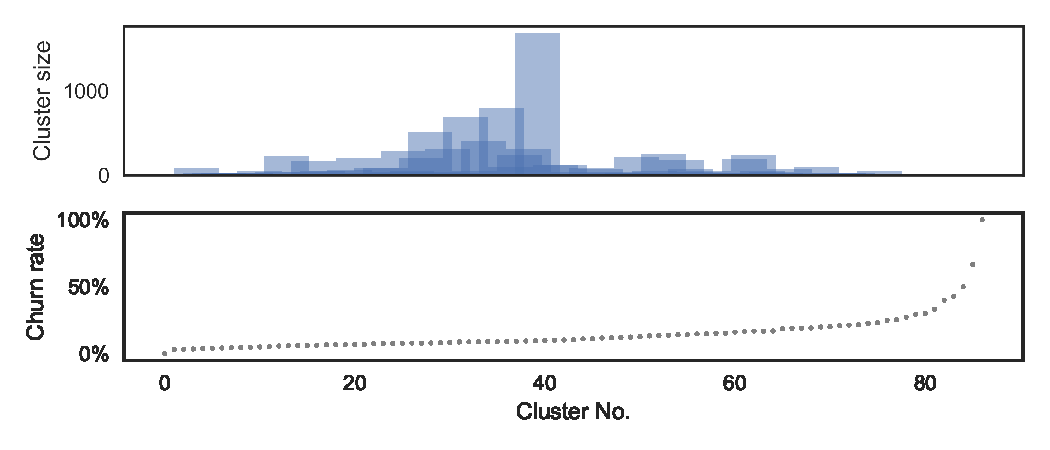
\includegraphics[scale=.7, trim={0 0 0 0}, clip]{ClusteringG3_Complete.pdf}
\caption{Identified clusters in G3, their average sizes and associated churn rate.}
\label{fig:clusteringG3Complete}
\end{figure}

\subsection{Assessing Churn Probability}

Because we have assumed that each pupil has independent behaviours from others, and that customer month are independent in leading to churn outcome, we can interpret the cluster churn rate as the probability of churn of each individual pupil in that cluster.

We do clustering (independent features, then multivariate features and finally combine) for G1, G2 and G3 separately, and then translate the cluster churn rate into the individual churn probability. This allows us to have the distribution of individual churn probabilities for G1, G2, G3 and the whole combined sample. This is shown in \Cref{fig:churnProb}.

\begin{figure}[!h]
\centering
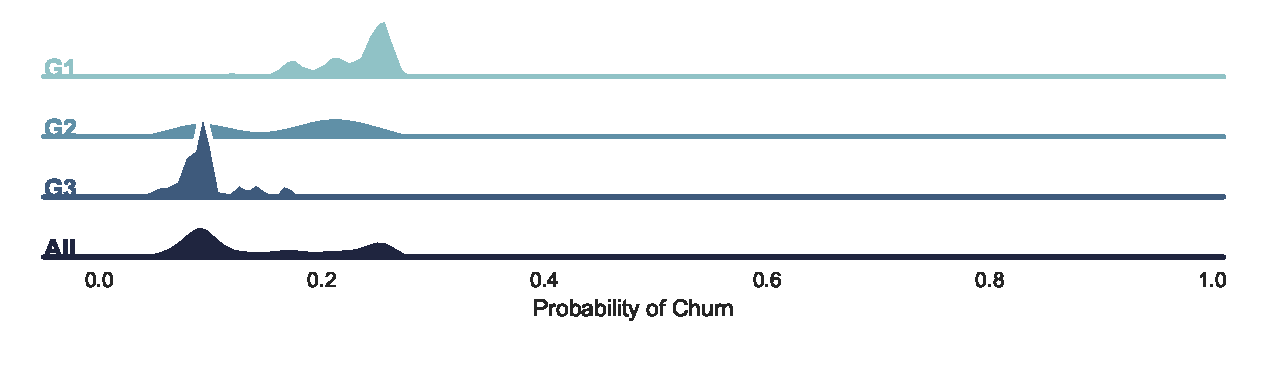
\includegraphics[scale=.7, trim={0 0 0 0}, clip]{ChurnProbability.eps}
\caption{Distribution (Gaussian kernel) of individual churn probability over pupils in G1, G2, G3 and in the whole combined sample. In making this plot, our algorithm and initialisation leads to 84 clusters for G1, 28 clusters for G2 and 268 clusters for G3.}
\label{fig:churnProb}
\end{figure}

Looking at the distribution for all pupils in the sample, we can observe a few concentrations of pupils centered at churn probabilities approximately 12\%, 25\%. If the behaviour based model does not work at all, the inferred churn probabilities will be purely random, which will converge to a normal distribution due to central limit theorem. Distributions shown in \Cref{fig:churnProb} are definitely not normal. This has shown that the behaviour based model has the predictive power to distinguish pupils with very different churn probabilities. In other words, pupils with the intention to churn exhibit different behaviours than those otherwise.

\subsection{Markov States Temporal Transition Analysis}

We will define the Markov states by grouping together clusters of similar level of churn rate because we want states to indicate different levels of churn risk. After forming states, we can compute transition probabilities.

\subsubsection{Defining Markov States}

In \Cref{fig:statesDefinition} we show an example definition of states. We choose to form 4 states $S_1$, $S_2$, $S_3$ and $S_4$ by grouping clusters according to 3 anchor points: 0.3, 0.22, 0.35 (the three vertical dashed line shown on the left plot). The state churn rates are 0.0\%, 11.7\%, 25.4\% and 55.6\% respectively. Therefore, we can say $S_1$ is the safest state where pupils in this state is very unlikely to churn. In contrast, $S_4$ is a very risky state in the sense that pupils in this state are 5.5 times more likely than average to cancel the subscription.

\begin{figure}[!h]
\centering
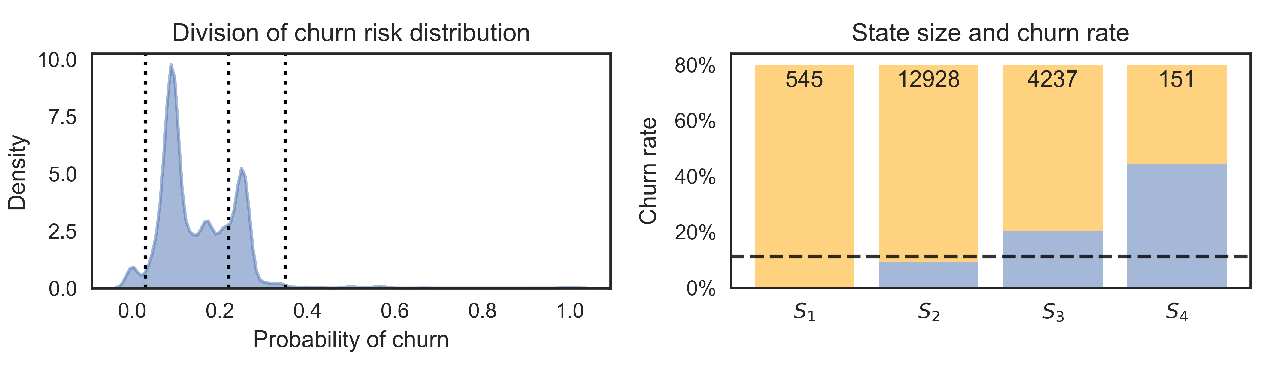
\includegraphics[scale=.7, trim={0 0 0 0}, clip]{StatesDefinition.pdf}
\caption{Defining Markov states by grouping together pupils of similar levels of churn risk. The right plot shows the size of each state as well as churn rate. The dashed line indicates the level of population churn rate.}
\label{fig:statesDefinition}
\end{figure}

The states' definition is dependent on the choice of anchor points. Whizz can choose the number and value of anchor points for forming states based on their needs. For example, if Whizz is interested in habits of very high-risk subscribers, they can increase the last anchor point.

When we want to check the churn risk for an active customer, we feed his feature data into the trained model and reach a churn probability. The predicted churn probability for a single customer might be very noisy and inaccurate due to overfitting in the clustering process. Overfitting means that the identified clusters can correspond too closely or exactly to the training data set, and therefore may fail to predict cluster for additional data point. However, when translating the churn probability into state, we are more confident about the accuracy of the predictive state. Therefore, defining state helps practical usage of the model in labeling and predicting churn risk levels.

\subsubsection{Transitional Analysis}

Following the state definitions in the previous section, we can move to the transitional analysis. We calculate the transition probabilities by formula (\ref{eq:transition}). Note that we need to add another state $S_\text{churn}$ which will only transit to itself (called an absorbing state, a state that once entered cannot be left). Hence, the complete state set is $\mathcal{S} = \{S_1, S_2, S_3, S_4, S_\text{churn}\}$.

We compute the transition probability matrix as:
\begin{equation}
A = 
\begin{bmatrix}
0.11 & 0.03 & 0.01 & 0.01 & 0.00 \\
0.66 & 0.68 & 0.33 & 0.28 & 0.00 \\
0.23 & 0.17 & 0.40 & 0.15 & 0.00 \\
0.00 & 0.00 & 0.01 & 0.01 & 0.00 \\
0.00 & 0.12 & 0.25 & 0.56 & 1.00 \\
\end{bmatrix},
\end{equation}
recall that $a_{pq} = \mathbb{P} (s_{t+1} = S_p | s_t = S_q)$. The transition probabilities are visualised in \Cref{fig:sankey} as a Sankey diagram. Churned pupils (those in $S_\text{churn}$) can not transit to other states. $S_2$ is the largest destination state, which makes sense as $S_2$ represents a ``normal'' state in which the churn probability is approximately the same as population average. Barely pupils transit from other states to $S_1$ (the safest state) or $S_4$ (the riskiest state). This seems imply two behavioural paths. First, if a pupil is very likely to stay live in the subscription (in $S_1$), then his intention of exit will be gradually accumulated since most likely he will transit to $S_2$ in the next period and $S_2$ again the next. Second, the reason for strong intention of churn might be purely external and irrelevant to customer experience at Whizz, since there is little chance of transiting to $S_4$.

\begin{figure}[!h]
\centering
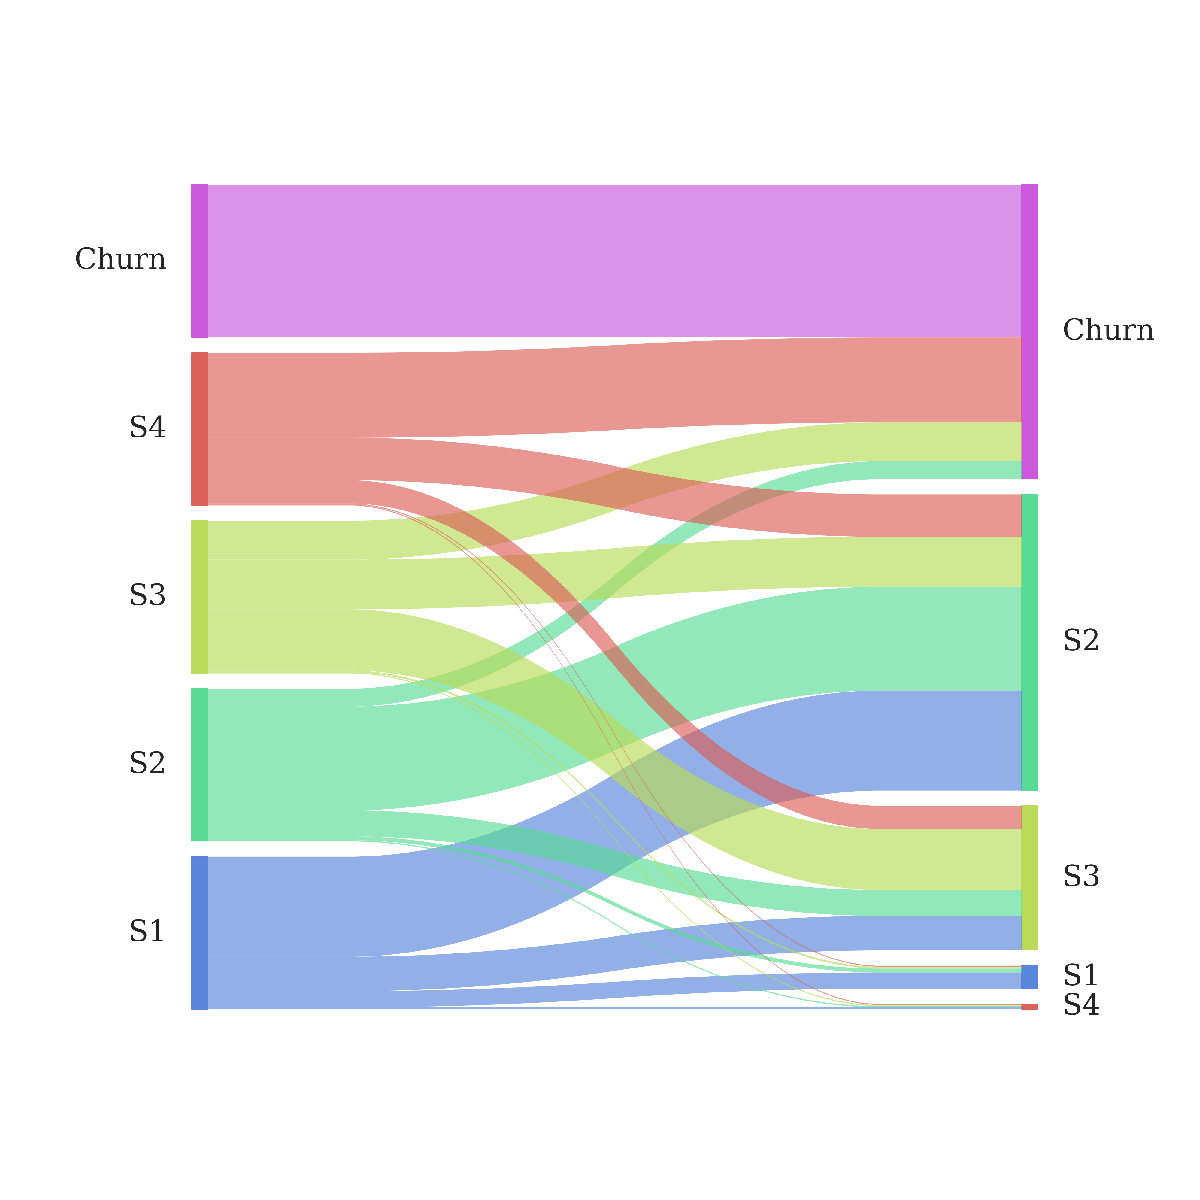
\includegraphics[scale=.5, trim={0 3cm 0 3cm}, clip]{Sankey.pdf}
\caption{Sankey diagram showing the transition probabilities between states from time $t$ to time $t+1$. The thickness of each band represents the magnitude of the transition probability from the state on the left to the state on the right.}
\label{fig:sankey}
\end{figure}

\subsection{Feature Impact}

We can examine how features play a role in differentiating the churn risk of pupils. A simple and useful examination is to compare how features distribute differently for different states. We have shown the distributions of multivariate features in \Cref{fig:ftrImpMulti}.

\begin{figure}[!h]
\centering
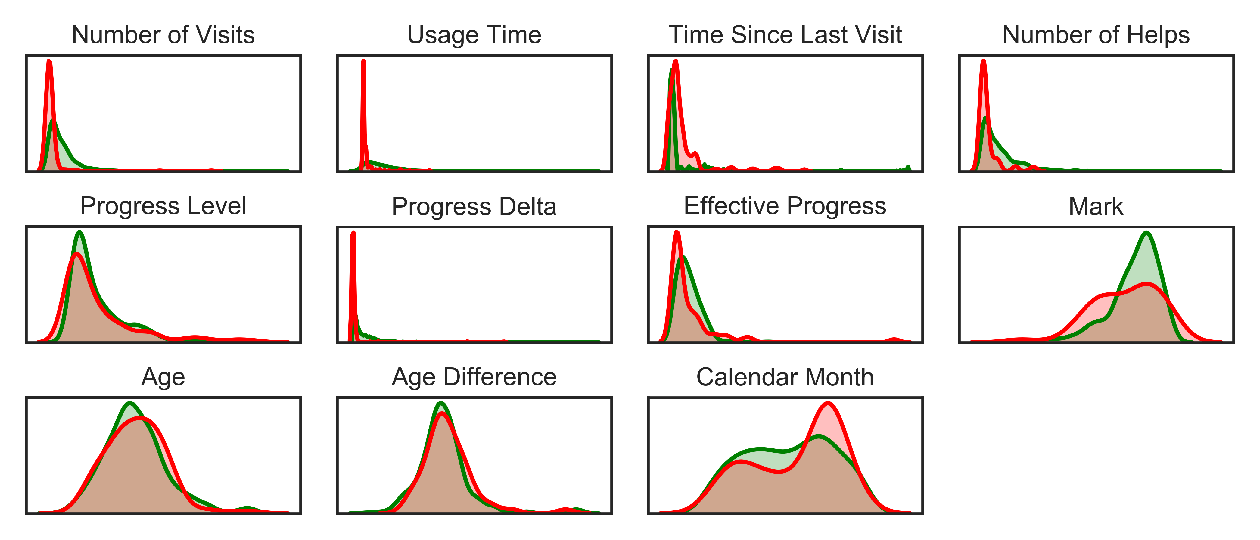
\includegraphics[scale=.7, trim={0 0 0 0}, clip]{FeatureImpactMultivariate.pdf}
\caption{Distributions of features for $S_1$ and $S_4$. We flag distribution for $S_1$, the safest state, by green color and $S_4$, the riskiest state, by red color.}
\label{fig:ftrImpMulti}
\end{figure}

Multiple implications can be drawn. If the red and green distributions of some feature do not deviate too much from each other, we can conclude that this feature might not be very informative of distinguishing the states. For example, age, age difference, progress level appear to be not informative. Mean and variations of the distributions are useful to tell how features influence churn risk. For example, pupils having more visits, or spending more time are less likely to churn. 

For each of the independent features, we can find the most frequent component for each state. This is shown in \Cref{fig:ftrImpIndep}. Pupils having a lot of exercises/lessons incomplete, no fail outcome, moderately high stack rate, full assessment are most likely to churn.

\begin{figure}[!h]
\centering
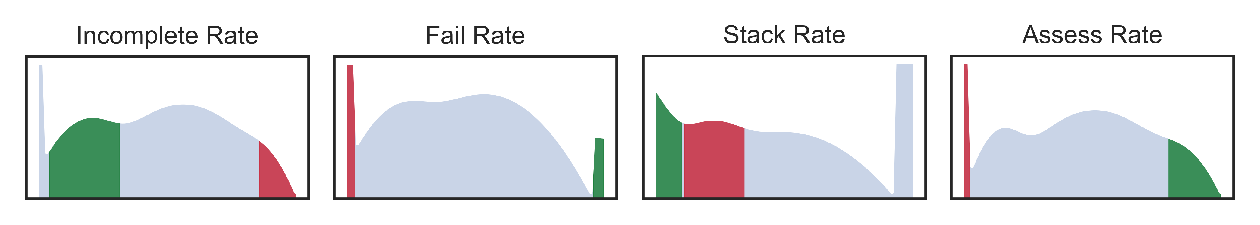
\includegraphics[scale=.7, trim={0 0 0 0}, clip]{FeatureImpactIndependent.pdf}
\caption{Distributions of features for $S_1$ and $S_4$. We flag the most frequent component for $S_1$, the safest state, by green color and $S_4$, the riskiest state, by red color. Note that the data for stack rate and assess rate are reversed by order.}
\label{fig:ftrImpIndep}
\end{figure}

